\documentclass[twocolumn,showpacs,%
  nofootinbib,aps,superscriptaddress,%
  eqsecnum,prd,notitlepage,showkeys,11pt]{article}

\usepackage{amssymb}
\usepackage{amsmath}
\usepackage{graphicx}
\usepackage{dcolumn}
\usepackage[hidelinks,colorlinks=true,linkcolor=blue,citecolor=blue]{hyperref}
\usepackage{titlesec}
\usepackage{minted}
\usepackage{authblk}
\usepackage{algorithm}
\usepackage{algpseudocode}
\usepackage{booktabs}
\usepackage[legalpaper, margin=1in]{geometry}
\frenchspacing
\setlength{\pdfpagewidth}{8.5in}
\setlength{\pdfpageheight}{11in}
\newcommand\headercell[1]{%
   \smash[b]{\begin{tabular}[t]{@{}c@{}} #1 \end{tabular}}}

\begin{document}

\title{Heuristics in the Longest Simple Path Problem}
\author[1]{Justin J. Xie}
\affil[1]{Institute for Computing in Research}
\date{}

\twocolumn[\begin{@twocolumnfalse}
\maketitle
\begin{abstract}
Finding the Longest Simple Path (LSP) in a unit-weighted undirected graph is an NP-Hard problem. We have explored the effectiveness of various heuristics for the LSP problem, and their potential for further use. In our exploration, we implemented heuristics inspired by well-known greedy techniques. Other heuristics utilized novel graph features to improve performance. We benchmarked the performance of these heuristics on accuracy, error, and speed on small random graphs. We found that these heuristics provided a considerable speed improvement to the na\"ive brute-force solution. We found that sparse graphs were the most difficult for our heuristics. This result supports other research indicating that sparse graphs continue to provide challenges for heuristics and approximation algorithms to solve.
\end{abstract}
\end{@twocolumnfalse}]  

\section{Introduction}

The Longest Simple Path (LSP) problem is a long-standing problem of both theoretical and practical interest. A path is simple if it does not repeat vertices. Finding the longest simple path in a graph involves finding the simple path with maximum length. 

Much work has been done on variations of the LSP problem. Solutions to the longest paths in directed, acyclic graphs and trees are the most commonly referenced and utilized solutions. In our research, we set out to explore the LSP problem in undirected unit-weighted connected graphs. The LSP problem is NP-hard: there is no existing solution or computer capable of finding the LSP of an arbitrary graph in polynomial time. As such, heuristic approximation might be an attractive alternative to searching for perfect solutions. In our research, we explored heuristics for this purpose.

Our main research contribution is the development and examination of high-level heuristics and principles of two different kinds: variations of the classic greedy approach, and heuristics involving constructing spanning trees from the graph in order to utilize Dijkstra's LSP algorithm for trees~\cite{club2002computing}. These heuristics classified a graph's vertices as "peripheral" and "central", using this classification along with other graph features to determine which edges to cut during tree construction.

We tried five heuristics that fall into one of the two categories mentioned above. We experimented with the implementation of these heuristics and obtained benchmark results that allow comparison to past and future explorations of the LSP problem. The data we gathered on these heuristics allowed us to gain some insight into sources of difficulty in LSP construction. We found that each heuristic had its own points of failure. The greedy algorithm failed to break ties; the graph pruning heuristic may not be cutting the most optimal edges. These issues can be further explored and possible remedies can be found for more efficient and accurate heuristics.

We found that when compared to past proposed greedy heuristics, our greedy heuristic showed similar behaviors when the number of edges in a graph was increased. It performed adequately in trees and denser graphs, where many solutions were available, but struggled with certain sparse graphs that only contained one or two possible longest simple paths. The graph pruning heuristics also showed promise for future use. On their own, they struggled to consistently cut the graph into a tree containing the longest simple path. 

Our research has shown that heuristics, although far faster than brute-force algorithms, often fail to account for the bigger picture. In our exploration of the LSP problem, the greedy and graph pruning/periphery heuristics that only registered and factored in data local to their ``current position'' in the graph required few calculations, making them faster. Longest simple paths, however, often require a view of the graph in its entirety in order to find the exact solution. Thus, heuristics that factor in all of the graph or make an extra calculation when deciding on a ``next vertex'' are the ones that outperformed in the accuracy category when compared to similar heuristics.

This is also the reason for the heuristics' improved ability to find longest paths on dense graphs in comparison to sparse graphs. Dense graphs give heuristics far more options for possible longest simple paths. As a result, even when the heuristics do not consider the entirety of the graph, the path they follow is more likely to be the LSP. In sparse graphs, there are often only one or two longest simple paths, where a single wrong turn in a heuristic's path will lead to an incorrect LSP. As has been confirmed by several other papers and their heuristics, the sparse graphs continue to be the more challenging aspect of implementing heuristics into the longest simple path problem.

\section{Background}

The longest simple path (LSP) in a graph is the longest possible path that originates at any vertex and traverses the graph without repeating vertices. The problem is an NP-Hard problem: there is no known algorithm capable of finding the LSP on an arbitrary graph in polynomial time. As the number of vertices and the size of the graph increases, any algorithm that guarantees an accurate solution hits an ``exponential wall'' where even the fastest and most optimized hardware struggle to efficiently identify the longest simple path in an efficient manner.

\section{Related Work} 
The longest simple path problem is a constantly revisited problem. While no general solution has been found, continual research into the problem has found polynomial-time solutions or even linear time solutions for many classes of graph.

One such class is the directed acyclic graph. The longest path of these graphs can be found in linear time by inverting each edge's weight and solving it as a shortest path problem using topological sort.~\cite{sedgewick_wayne_2017}

Trees---undirected, acyclic graphs---are solvable in linear time using an algorithm by Dijkstra that we call the ``Dijkstra Dangle''. This algorithm finds two ``extremes" of a tree using two breadth first searches: the path between them is the LSP for the tree~\cite{club2002computing}.

Block graphs and weighted trees have been shown to have linear time solutions; Cacti graphs in $\mathcal{O}(n^2)$ time~\cite{uehara2004efficient, uehara2007computing}. Bipartite Permutation graphs, too, have an $\mathcal{O}(n)$ solution~\cite{uehara2007linear}. Interval graphs are solvable in $\mathcal{O}(n^4)$ time~\cite{ioannidou2009longest,  giannopoulou2015polynomial}, Circular-Arc graphs in $\mathcal{O}(n^4)$ time~\cite{mertzios2011computing}, Co-Comparability graphs in $\mathcal{O}(n^4)$ time~\cite{mertzios2012simple}, and Ptolemaic graphs in $\mathcal{O}(n^5)$ time~\cite{takahara2008longest}.

The LSP problem on general graphs has been intensively studied by many. One notable approach is dynamic programming using graph partitioning~\cite{balyo2017optimal}, including parallelization~\cite{fieger2019finding}. Another approach uses constraint programming, with both an exact algorithm and a tabu local-search algorithm: this is more successful in niche groups of graphs~\cite{pham2012solving}.

Approximations and heuristics for LSP have also been a big consideration. Approximation has been applied to specific graph groups without polynomial time solutions, such as grid graphs~\cite{zhang2011approximating}, (approximated in $O({n^2})$ time), and also to more general cases. Examples of approximation algorithms include genetic algorithms~\cite{mathew2012genetic, portugal2010study, scholvin1999approximating}, a color-coding~\cite{alon1995color} inspired approximation~\cite{scutella2003approximation}, a simulated annealing algorithm~\cite{scholvin1999approximating}, and a tabu-search algorithm~\cite{scholvin1999approximating}.

Two heuristic approaches similar to ours were a graph pruning heuristic and a greedy variation heuristic. A permissible grid-graph pruning heuristic was used with A* and Depth-First Branch-and-Bound complete search algorithms to find the LSP~\cite{cohen2020solving}. A greedy variation heuristic called the \textit{k}-step Greedy Lookahead employed a method of finding partial paths by looking \textit{k} vertices ahead~\cite{scholvin1999approximating}.

\section{Heuristics}

We developed several heuristic approximations to LSP for undirected unit-weighted connected graphs. These heuristics employed past techniques, such as the greedy or pruning algorithms, but utilized different graph characteristics. In the process of applying and testing our heuristics, we confirmed properties of the LSP problem introduced in previous work. We also discovered certain graph characteristics that could be helpful for future work.

\subsection{Greedy Heuristics}

The first group of heuristics that were explored were ones based on the classic greedy algorithm. These algorithms depend on making the ``best'' decision in the current situation. In order to utilize this principle, there needed to be a graph characteristic that was identifiable and able to be recalculated on a local scale. This led us to the graph characteristic of vertex neighbor counts. A vertex neighbor count is the number of vertices adjacent to the vertex whose neighbor count is being calculated. This was a feature of the graph that could be recomputed every step.

\begin{algorithm*}
\begin{algorithmic}

\State let $G$ be the given graph
\State longest\_path $\gets$ empty path
\For{vertex in $G$}
    \State current\_path $\gets$ empty path
    \While{adjacent vertices to last vertex exist}
        \If {$V$ with least neighbors and neighbor count $>$ 1}
            \State add $V$ to current\_path
        \ElsIf {$V$ with neighbor count $=$ 1}
            \State add $V$ to current\_path
        \Else
            \State end traversal
        \EndIf
    \EndWhile
    \If {length of current\_path $>$ length of longest\_path}
        \State longest\_path $\gets$ current\_path
    \EndIf
\EndFor
\State return vertices\_visited - 1

\end{algorithmic}
\caption{Greedy Neighbor Heuristic}\label{alg:GreedyNeighbor}
\end{algorithm*}

The greedy heuristic utilizing the graph's vertex neighbor count feature, or the Greedy Neighbor heuristic, found the longest simple path in a graph by starting at each vertex. It would then traverse the graph by choosing adjacent vertices with the least available neighbors until there were no options left. Each step in the traversal required a recalculation of the available vertices along with their neighbor count. Each starting node would eventually end up with a greedy traversal of the graph, which was then used to calculate the greedy path from each vertex. Finally, the longest greedy path was output as the heuristics solution to the LSP problem in the given graph.

The greedy heuristic was based on the options for the next vertex in traversing the graph. The heuristic would prioritize visiting vertices with fewer neighbors and thus a lower number of ``options'' by which it could be reached. Consequentially, vertices with more neighbors were visited later, as there were more ``options'' to get to them. The problem with this heuristic was that it was often in a position where two or more vertices adjacent to the current vertex had the same number of available neighbors, putting the heuristic at a crossroads of tie breaking. In our first iteration of the Greedy Neighbor heuristic, the vertex with a lower ID was chosen. While this sometimes was inconsequential, because in many cases both paths led to longest paths being found, there were also graphs where choosing the lower node ID led to a shorter path length than the desired LSP. This behavior was most noticeable in larger and sparse graphs with seven or more vertices. There needed to be a tiebreaker that could pick the correct choice instead of letting chance decide. 

The second version of the Greedy Neighbor heuristic involved a Depth-First-Search (DFS) that acted as the tiebreaker when more than one adjacent vertex had the most neighbors. This DFS was a specialized version that traversed the remaining available vertices in the graph. It prioritized visiting vertices with lower IDs (instead of randomly deciding the next vertex). For each of the tied adjacent vertices, it created a tree graph with the root being the starting DFS vertex. For each vertex that had tied with having the most neighbors, the specialized DFS was executed to create post-DFS trees. The internal path length is the sum of the depth (distance from root) of all nodes. The internal path length of each post-DFS tree was calculated and the one with the highest was chose as the next vertex to visit in the greedy traversal. 

\subsection{Graph Centrality, Periphery, and Pruning}

The second group of heuristics was based on the centrality of the vertices. The definition of three key terms representing graph and vertex centrality are as follows:

\begin{enumerate}
    \item \textbf{Vertex Periphery}: For any vertex \textit{v}, the vertex periphery (VP) is the longest shortest path from \textit{v} to any other vertex. The lower the vertex periphery of \textit{v}, the more central \textit{v} is.

    \item \textbf{Total Vertex Periphery}:  For any vertex \textit{v}, the total vertex periphery (TVP) is the sum of all shortest paths from \textit{v} to every other vertex. The lower the total vertex periphery of \textit{v}, the more central \textit{v} is. Figure~\ref{fig:GraphTVPGradient} gives a visual illustration of TVP.

    \item \textbf{Graph Periphery}: For any graph \textit{G}, the graph periphery (GP) is the sum of the TVP of all vertices in \textit{G}.
\end{enumerate}

\begin{figure}
    \centering
    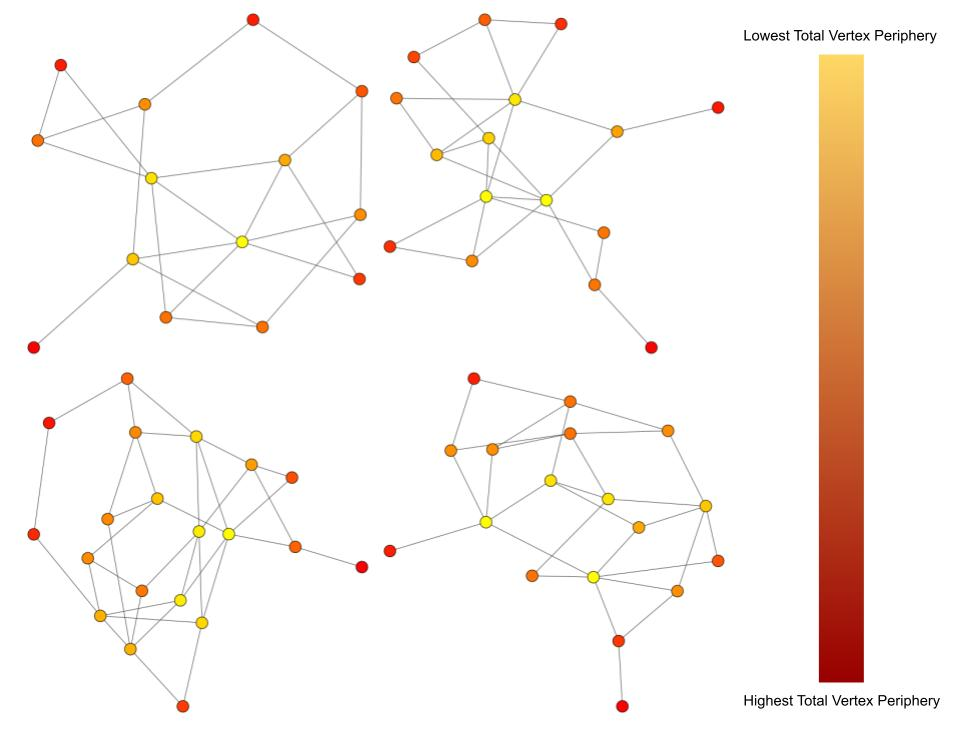
\includegraphics[width=0.8\linewidth]{GraphTVPGradientsExamples.jpg}
    \caption{Example Graphs With Gradient Representation of Total Vertex Periphery}
    \label{fig:GraphTVPGradient}
\end{figure}

All graph centrality heuristics were based on the idea that given a graph \textit{G} with \textit{n} vertices and \textit{m} edges, if you cut specific \(m - (n - 1)\) edges, the graph would then be pruned into a tree \textit{T}, whose longest path corresponds to the longest path in \textit{G}. The longest path of \textit{T} could then be found in linear time with Dijkstra's Dangle algorithm.

The first graph centrality heuristic was one that made use of the TVP values. Named the Prune Central Edges heuristic, it relied on the assumption that the edges connecting vertices with lower TVP (meaning that they were more central edges) were unnecessary in the LSP of the graph. However, that proved to be an incorrect assumption because during testing, it was found that in certain instances, the edge connecting vertices with the lowest TVP was utilized in the longest simple path.

\begin{algorithm}
\begin{algorithmic}

\State let $n$ be the number of vertices 
\State let $m$ be the number of edges
\State let $G$ be the given graph
\State{}
\For {$m - (n - 1)$ cuts}
    \State $M \gets$ mapping of vertex TVP
    \State $V \gets$ vertex with lowest TVP
    \For {neighbors of $V$}
        \State $E \gets$ edge from $V$ to neighbor
        \State temporarily remove $E$
        \If {$G$ is connected}
            \State remove $E$ from $G$
        \Else
            \State next edge
        \EndIf
    \EndFor
\EndFor
\State{}
\State execute Dijkstra's Dangle on cut graph
\State return longest path obtained by Dijkstra's
\end{algorithmic}
\caption{Prune Central Edges}\label{alg:PruneCentralEdges}
\end{algorithm}

The second graph centrality heuristic also made use of the total vertex periphery values. The Stretch Lowest TVP heuristic worked by choosing a vertex \textit{v} with the lowest TVP that had available edges that could be removed without disconnecting the graph. Next, the heuristic would find and cut the edge connecting to \textit{v} that, when removed, would increase the TVP of \textit{v} the most. This heuristic operated under the idea that the optimal tree---containing the longest path---would have the highest possible graph periphery. By removing edges from the vertices with low TVP, the heuristic would be increasing the TVP of the vertices and stretching the GP of the graph.

\begin{algorithm}
\begin{algorithmic}

\State let $n$ be the number of vertices 
\State let $m$ be the number of edges
\State{}
\For {$m - (n - 1)$ cuts}
    \State $V$ $\gets$ vertex with lowest TVP
    \State initialize highest periphery
    \For {edge connected to $V$}
        \State temporarily remove edge
        \State find TVP
        \If {TVP $>$ highest periphery}
            \State {highest periphery $\gets$ TVP}
        \EndIf
    \State remove edge with highest periphery
    \EndFor
\EndFor
\State{}
\State execute Dijkstra's Dangle on cut graph
\State return longest path obtained by Dijkstra's
\end{algorithmic}
\caption{Stretch Lowest TVP}\label{alg:StretchLowestTVP}
\end{algorithm}

Through our testing, it was found that in certain graphs, the edges that would increase the TVP of a vertex were edges that were a crucial part of the graph's LSP. As a result, the principle that this exact heuristic followed was not the correct way to go about cutting the graph into a tree.

The third graph centrality heuristic made use of the graph periphery (GP). The Stretch Graph Periphery heuristic operated by looping through all removable edges (ones that did not create discontinuities in the graph) and finding the one that brought about the largest increase in the GP when removed. Similar to the Stretch Lowest TVP heuristic, the Stretch Total Graph heuristic also worked to remove edges that lowered the graph periphery and to stretch the graph out to its widest possible tree. 

\begin{algorithm}
\begin{algorithmic}

\State let $n$ be the number of vertices 
\State let $m$ be the number of edges
\State let $G$ be the given graph
\State{}
\For {$m - (n - 1)$ cuts}
    \State initialize highest periphery
    \For {all edges in $G$}
        \State temporarily remove edge
        \State $P \gets$ graph periphery
        \If {$P >$ highest periphery}
            \State {highest periphery $\gets P$}
        \EndIf
    \State remove edge with highest periphery
    \EndFor
\EndFor
\State{}
\State execute Dijkstra's Dangle on cut graph
\State return longest path obtained by Dijkstra's
\end{algorithmic}
\caption{Stretch Graph Periphery}\label{alg:StretchGraphPeriperhy}
\end{algorithm}


Similar to the Stretch Lowest TVP heuristic, it was revealed that there were graphs that did not work well for the Stretch Total Graph heuristic. There were certain graphs where the edge that increased the GP the most were part of the longest simple path. Other graphs had edges that increased the GP the same. With no tiebreaker method, the edge with lower vertex IDs would be chosen to be removed. As such, there were graphs where necessary edges were removed because of ties between edges.

\section{Experimental Results}

As we designed our heuristics, we experimented with prototype implementations. We eventually constructed a benchmark suite for a more thorough evaluation.

\subsection{Experiment Setup}

In order to implement our heuristics, we utilized the Python programming language (version 3.10.4) and its \texttt{igraph} package. The \texttt{igraph} package contains an extensive array of functions and variable types fit for quick and efficient manipulation as well as useful graph visualization tools. We utilized \texttt{igraph}'s ability to quickly add and remove edges and vertices, as well as its functions for plotting graphs and returning important graph characteristics such number of edges, vertices, or a vertex's neighbors. The package also included functions such as \verb+get_simple_paths+ or \verb+shortest_paths+ that made the translation of heuristics from idea to code a straightforward process.

We used \texttt{igraph}'s visualization tools to draw nicely-layed-out graphs such as the one in Figure~\ref{fig:ExampleGraph}.  Working with graphs that were visualized this way helped to in understanding different implementations of heuristics like the greedy heuristic and new characteristics.

\begin{figure}
    \centering
    \includegraphics[width=0.8\linewidth]{examplegraph.png}
    \caption{Example Graph, Drawn by Python-igraph}
    \label{fig:ExampleGraph}
\end{figure}

\subsection{Experimental Approach}

The first step in implementing heuristics was the proof-of-concept. By looking at characteristics of a graph, we were able to find some that might be of use in a heuristic. Characteristics such as vertex neighbor count, diameter of the graph, and vertex centrality were all examples of graph characteristics that were involved in one or more heuristics. We often used graph features for inspiration when pondering possible heuristics.

When heuristic ideas revealed themselves to be feasible and capable of attaining accurate longest simple paths, pseudocode was written to be used in the second step: Python implementation. This was where the ideas were implemented as heuristics compatible with \texttt{igraph} for testing.

\subsection{Random Graph Generation}

The random graphs for visualization and benchmarking were created through a randomization process called Tree-Based-Graph-Gen. This algorithm, given a \textit{n} vertices and \textit{m} edges, creates a random, undirected, connected graph by creating a tree with all \textit{n} vertices and \(n-1\) edges. The remaining \(m - (n - 1)\) required edges are then added randomly throughout the graph.

\begin{algorithm}
\begin{algorithmic}

\State let $E$ be a set of all possible edges ($i$, $j$)
\For{vertex $i$ from $2$ to $n$}
    \State let $j$ be a random number from $i$ to $(i - 1)$
    \State connect $i$ to $j$
    \State remove ($i$, $j$) from $E$
\EndFor
    
\For{$m - (n - 1)$ edges}
    \If{$E$ is empty}
        \State return fail
    \EndIf
    \State pick random edge $(i - 1)$ from $E$
    \State connect $i$ to $j$
    \State remove ($i$, $j$) from $E$
\EndFor

\end{algorithmic}
\caption{A random graph generation algorithm}\label{alg:RGG}
\end{algorithm}

This ``random'' graph generation, however, is not truly random. Due to the way that the algorithm chooses ``random" target edges during the base-tree creation phase, certain graph shapes are more likely to be built than others. 

\subsection{Benchmarking Methods}
For the testing and benchmarking of our heuristics, we created three tests to measure crucial areas of the Longest Simple Path Problem: accuracy, error, and runtime. For consistency, the graphs used throughout all tests were the same graphs. The tests were as follows:

\begin{enumerate}
    \item \textbf{Accuracy:} The percentage of graphs that a given heuristic gets the exact longest simple paths for.
    \item \textbf{Error:} The average difference between the actual longest simple path and longest simple path found by a given heuristic.
    \item \textbf{Runtime:} The wall-clock average execution time of a given heuristic over a group of graphs.
\end{enumerate}

\subsection{Experimental Results}

\begin{table*}[htp]
\caption{Heuristics Accuracy on 9-Vertex Graphs}
\centering
\small
\noindent
\begin{tabular}{@{} *{6}{c} @{}}
\headercell{Number of \\ Edges} & \multicolumn{5}{c@{}}{Heuristics}\\
\cmidrule(l){2-6}
& greedy & dfs\_greedy & prune\_central & stretch\_total & stretch\_nodes \\
\hline
 8 & 100.0 & 100.0 & 100.0 & 100.0 & 100.0 \\
 9 & 99.0 & 100.0 & 98.0 & 99.0 & 99.0 \\
 10 & 99.0 & 100.0 & 96.0 & 91.0 & 92.0 \\
 11 & 99.0 & 98.0 & 92.0 & 90.0 & 90.0 \\
 12 & 100.0 & 100.0 & 91.0 & 78.0 & 84.0 \\
 13 &100.0 & 99.0 & 83.0 & 79.0 & 81.0 \\
 14 & 99.0 & 100.0 & 92.0 & 86.0 & 88.0 \\
 15 & 99.0 & 100.0 & 86.0 & 84.0 & 86.0 \\
 16 & 100.0 & 100.0 & 91.0 & 88.0 & 81.0 \\ 
 17 & 100.0 & 100.0 & 98.0 & 88.0 & 89.0 \\
 18 & 100.0 & 100.0 & 96.0 & 96.0 & 87.0 \\
 19 & 100.0 & 100.0 & 98.0 & 96.0 & 91.0 \\
 20 & 100.0 & 100.0 & 100.0 & 99.0 & 95.0 \\
 21 & 100.0 & 100.0 & 99.0 & 99.0 & 94.0 \\
 22 & 100.0 & 100.0 & 99.0 & 98.0 & 97.0 \\
 23 & 100.0 & 100.0 & 100.0 & 94.0 & 96.0 \\
 24 & 100.0 & 100.0 & 100.0 & 100.0 & 96.0 \\
 25 & 100.0 & 100.0 & 100.0 & 97.0 & 96.0 \\
 26 & 100.0 & 100.0 & 100.0 & 99.0 & 95.0 \\
 27 & 100.0 & 100.0 & 100.0 & 100.0 & 97.0 \\
 28& 100.0 & 100.0 & 100.0 & 99.0 & 94.0 \\
 29 & 100.0 & 100.0 & 100.0 & 100.0 & 97.0 \\
 30& 100.0 & 100.0 & 100.0 & 100.0 & 94.0 \\
 31 & 100.0 & 100.0 & 100.0 & 100.0 & 98.0 \\
 32 & 100.0 & 100.0 & 100.0 & 100.0 & 96.0 \\
 33 & 100.0 & 100.0 & 100.0 & 100.0 & 98.0 \\
 34 & 100.0 & 100.0 & 100.0 & 100.0 & 100.0 \\
 35 & 100.0 & 100.0 & 100.0 & 100.0 & 100.0 \\
 36 & 100.0 & 100.0 & 100.0 & 100.0 & 100.0 
\end{tabular}
\end{table*}

\begin{figure*}[htp]
    \centering
    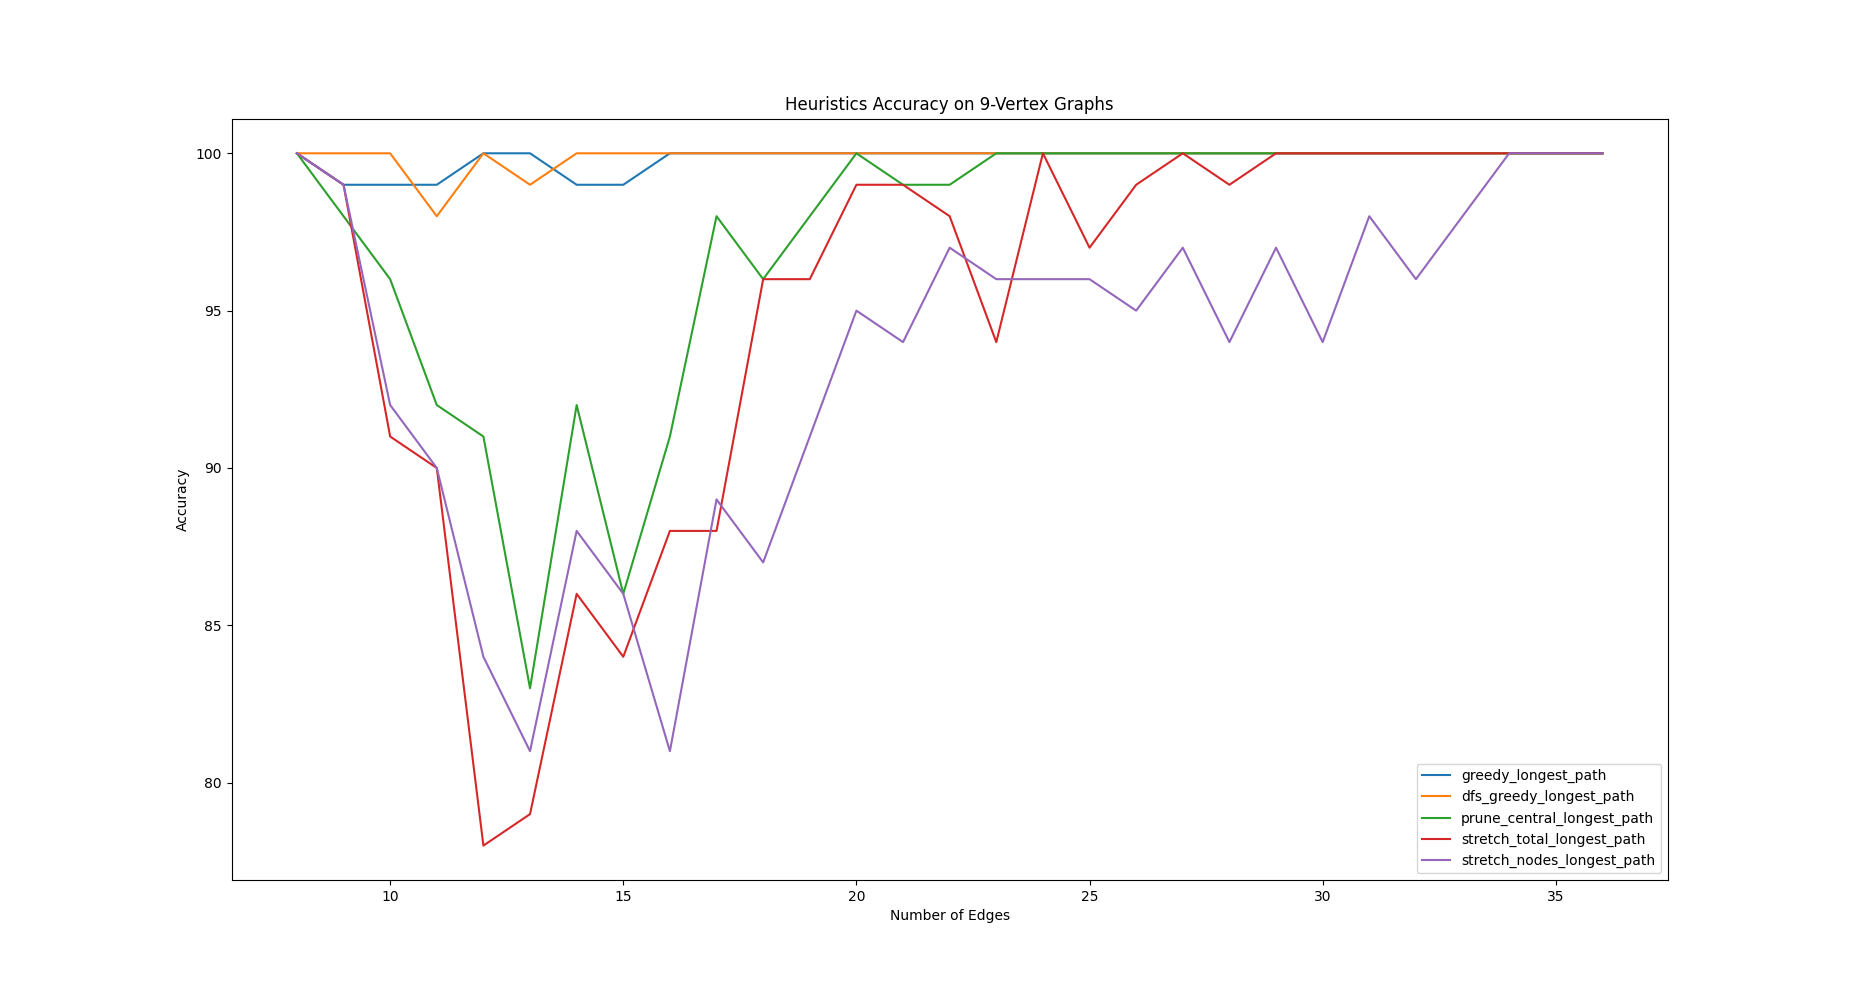
\includegraphics[width=\linewidth]{Accuracy9VertexAll.png}
    \caption{Heuristics Accuracy on Graphs with 9 Vertices}
    \label{fig:Accuracy}
\end{figure*}

\begin{table*}[htp]
\caption{Heuristics Error on 9-Vertex Graphs}
\centering
\small
\noindent
\begin{tabular}{@{} *{6}{c} @{}}
\headercell{Number of \\ Edges} & \multicolumn{5}{c@{}}{Heuristics} \\
\cmidrule(l){2-6}
& greedy & dfs\_greedy & prune\_central & stretch\_total & stretch\_nodes \\
\hline
 8 & 0.0 & 0.0 & 0.0 & 0.0 & 0.0 \\
 9 & 0.01 & 0.0 & 0.02 & 0.01 & 0.01 \\
 10 & 0.01 & 0.0 & 0.04 & 0.09 & 0.08 \\
 11 & 0.01 & 0.02 & 0.08 & 0.10 & 0.10 \\
 12 & 0.0 & 0.0 & 0.09 & 0.23 & 0.16 \\
 13 & 0.0 & 0.01 & 0.18 & 0.21 & 0.19 \\
 14 & 0.01 & 0.0 & 0.08 & 0.14 & 0.12 \\
 15 & 0.01 & 0.0 & 0.14 & 0.16 & 0.14 \\
 16 & 0.0 & 0.0 & 0.19 & 0.13 & 0.19 \\ 
 17 & 0.0 & 0.0 & 0.02 & 0.12 & 0.11 \\
 18 & 0.0 & 0.0 & 0.04 & 0.04 & 0.13 \\
 19 & 0.0 & 0.0 & 0.02 & 0.05 & 0.09 \\
 20 & 0.0 & 0.0 & 0.0 & 0.01 & 0.05 \\
 21 & 0.0 & 0.0 & 0.01 & 0.01 & 0.06 \\
 22 & 0.0 & 0.0 & 0.01 & 0.02 & 0.03 \\
 23 & 0.0 & 0.0 & 0.0 & 0.06 & 0.04 \\
 24 & 0.0 & 0.0 & 0.0 & 0.0 & 0.04 \\
 25 & 0.0 & 0.0 & 0.0 & 0.03 & 0.04 \\
 26 & 0.0 & 0.0 & 0.0 & 0.01 & 0.05 \\
 27 & 0.0 & 0.0 & 0.0 & 0.0 & 0.03 \\
 28 & 0.0 & 0.0 & 0.0 & 0.01 & 0.06 \\
 29 & 0.0 & 0.0 & 0.0 & 0.0 & 0.03 \\
 30 & 0.0 & 0.0 & 0.0 & 0.0 & 0.06 \\
 31 & 0.0 & 0.0 & 0.0 & 0.0 & 0.02 \\
 32 & 0.0 & 0.0 & 0.0 & 0.0 & 0.04 \\
 33 & 0.0 & 0.0 & 0.0 & 0.0 & 0.02 \\
 34 & 0.0 & 0.0 & 0.0 & 0.0 & 0.0 \\
 35 & 0.0 & 0.0 & 0.0 & 0.0 & 0.0 \\
 36 & 0.0 & 0.0 & 0.0 & 0.0 & 0.0 \\
\end{tabular}
\end{table*}

\begin{figure*}[htp]
    \centering
    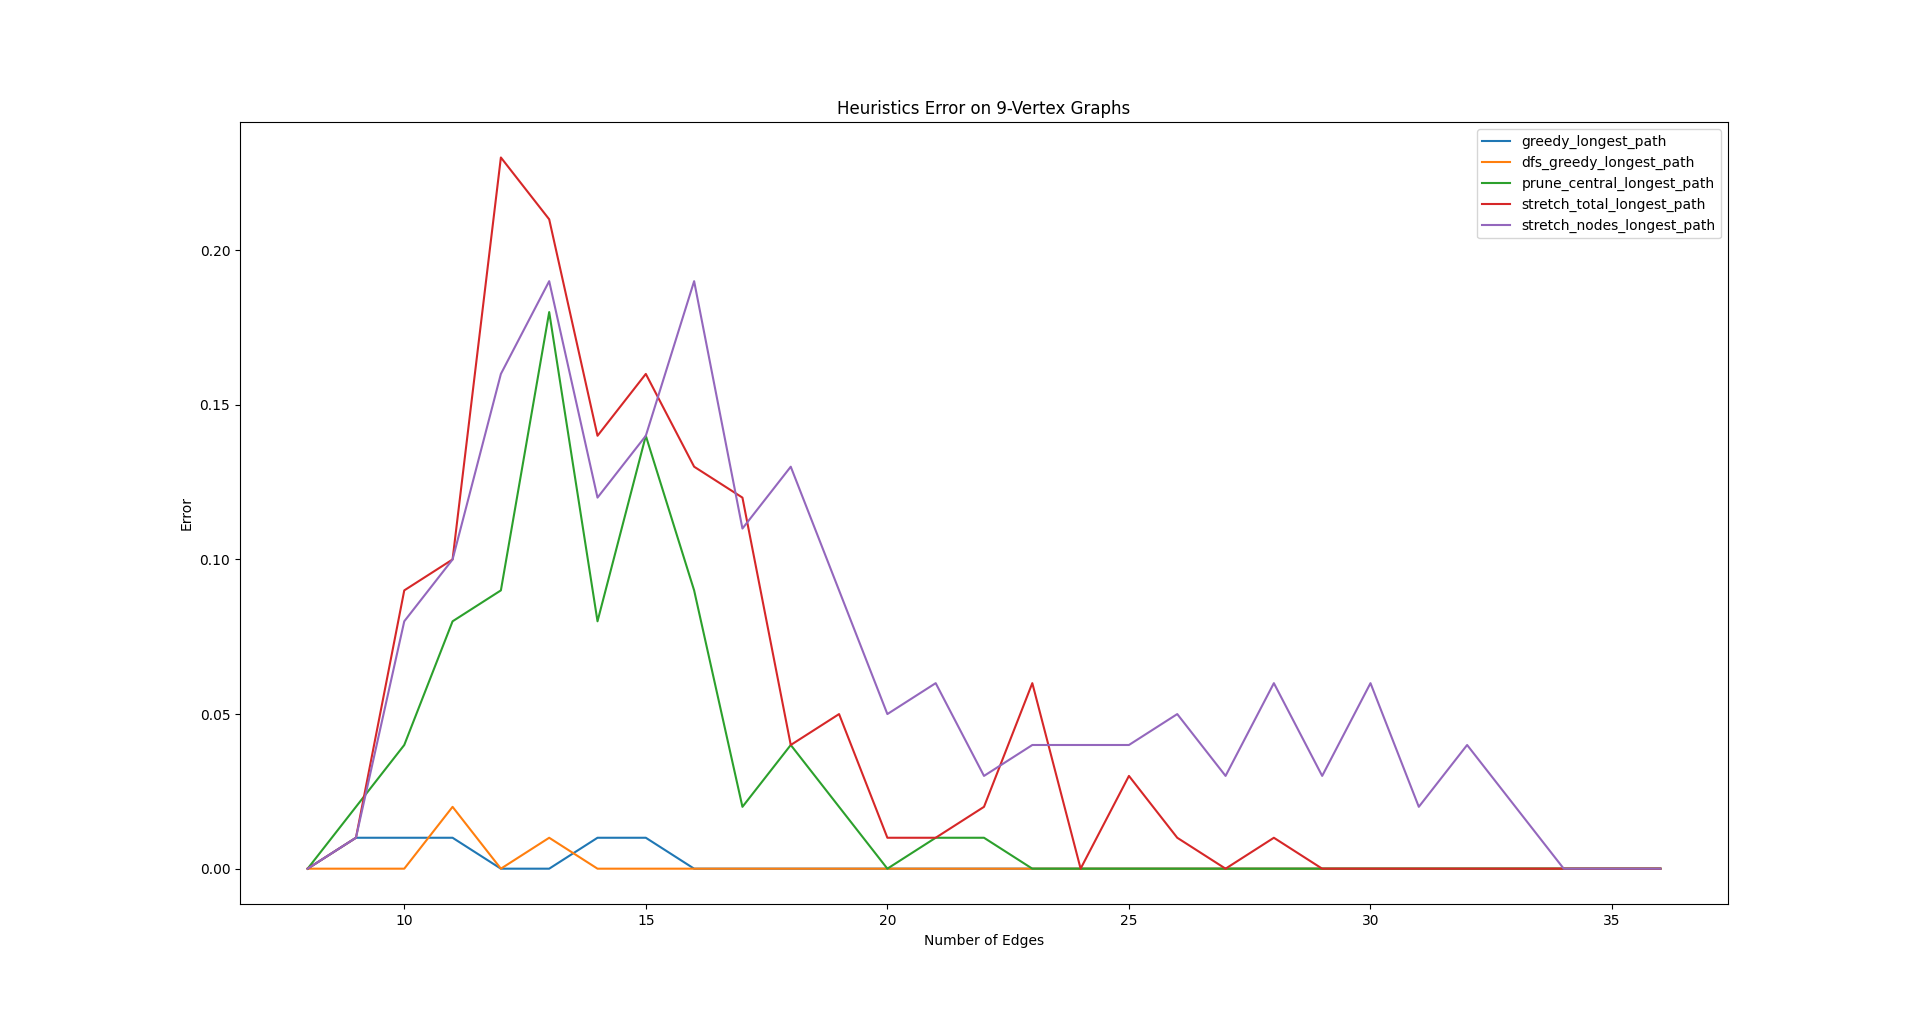
\includegraphics[width=\linewidth]{Error9VertexAll.png}
    \caption{Heuristics Error on Graphs with 9 Vertices}
    \label{fig:Error}
\end{figure*}

\begin{table*}[htp]
\caption{Heuristics Runtime on 9-Vertex Graphs}
\centering
\small
\noindent
\begin{tabular}{@{} *{7}{c} @{}}
\headercell{Number of \\ Edges} & \multicolumn{6}{c@{}}{Heuristics} \\
\cmidrule(l){2-6}
& greedy & dfs\_greedy & prune\_central & stretch\_total & stretch\_nodes & brute-force \\
\hline
 8 & 0.0001339 & 0.0002115 & 1.78E-05 & 1.24E-05 & 1.28E-05 & 3.93E-05 \\
 9 & 9.44E-05 & 0.0003868 & 0.0002032 & 0.0011236 & 0.0003383 & 5.81E-05 \\
 10 & 0.0001048 & 0.0005775 & 0.0004151 & 0.0023543 & 0.0006561 & 9.03E-05 \\
 11 & 0.0001125 & 0.0007197 & 0.0005731 & 0.0037371 & 0.0009669 & 0.0001347 \\
 12 & 0.0001214 & 0.0008422 & 0.0008724 & 0.0053146 & 0.0013564 & 0.0002133 \\
 13 & 0.0001287 & 0.0009806 & 0.0009262 & 0.0071409 & 0.0016779 & 0.0003941 \\
 14 & 0.000135 & 0.0011354 & 0.0011374 & 0.0090412 & 0.0020774 & 0.000534 \\
 15 & 0.0001397 & 0.0013132 & 0.0012995 & 0.0109298 & 0.0024597 & 0.000801 \\
 16 & 0.0001446 & 0.0013653 & 0.0014624 & 0.0131174 & 0.00292 & 0.0011781 \\
 17 & 0.0001484 & 0.0015664 & 0.0016971 & 0.015527 & 0.0033403 & 0.0017935 \\
 18 & 0.0001527 & 0.0017702 & 0.0018301 & 0.0182468 & 0.0038113 & 0.0027262 \\
 19 & 0.0001562 & 0.0020146 & 0.0020375 & 0.0209624 & 0.0043504 & 0.0043898 \\
 20 & 0.0001597 & 0.002153 & 0.0021626 & 0.0235532 & 0.0048087 & 0.0065727 \\
 21 & 0.0001618 & 0.0023596 & 0.0023787 & 0.0255448 & 0.0053355 & 0.0092391 \\
 22 & 0.0001643 & 0.00258 & 0.0025342 & 0.0292619 & 0.0058146 & 0.0133933 \\
 23 & 0.0001676 & 0.0027988 & 0.0027264 & 0.0325536 & 0.0064107 & 0.0192997 \\
 24 & 0.0001705 & 0.0030494 & 0.0030376 & 0.0360228 & 0.0069574 & 0.025796 \\
 25 & 0.0001729 & 0.0033103 & 0.0029793 & 0.0395946 & 0.0075332 & 0.03686 \\
 26 & 0.0001746 & 0.0034828 & 0.0031932 & 0.0434956 & 0.0080365 & 0.0492349 \\
 27 & 0.0001771 & 0.0037537 & 0.0033473 & 0.0471843 & 0.0085708 & 0.0655757 \\
 28 & 0.0001789 & 0.0040668 & 0.0034598 & 0.0520643 & 0.0092661 & 0.0890664 \\
 29 & 0.0001811 & 0.0044 & 0.0035829 & 0.0569198 & 0.0097569 & 0.1137601 \\
 30 & 0.0001832 & 0.0047944 & 0.0037833 & 0.0620864 & 0.0103405 & 0.1465667 \\
 31 & 0.0001856 & 0.0052211 & 0.0040176 & 0.0665662 & 0.0112145 & 0.1921401 \\
 32 & 0.0001874 & 0.0057643 & 0.0041552 & 0.0722577 & 0.011959 & 0.2542703 \\
 33 & 0.0001889 & 0.0063387 & 0.0044217 & 0.0775441 & 0.0127085 & 0.3268791 \\
 34 & 0.0001915 & 0.0074702 & 0.0045202 & 0.0832664 & 0.013976 & 0.4175168 \\
 35 & 0.000193 & 0.0085568 & 0.0046966 & 0.08821 & 0.0146478 & 0.5437159 \\
 36 & 0.0001936 & 0.010597 & 0.0053172 & 0.0936378 & 0.0153948 & 0.7104294
\end{tabular}
\end{table*}

\begin{figure*}[htp]
    \centering
    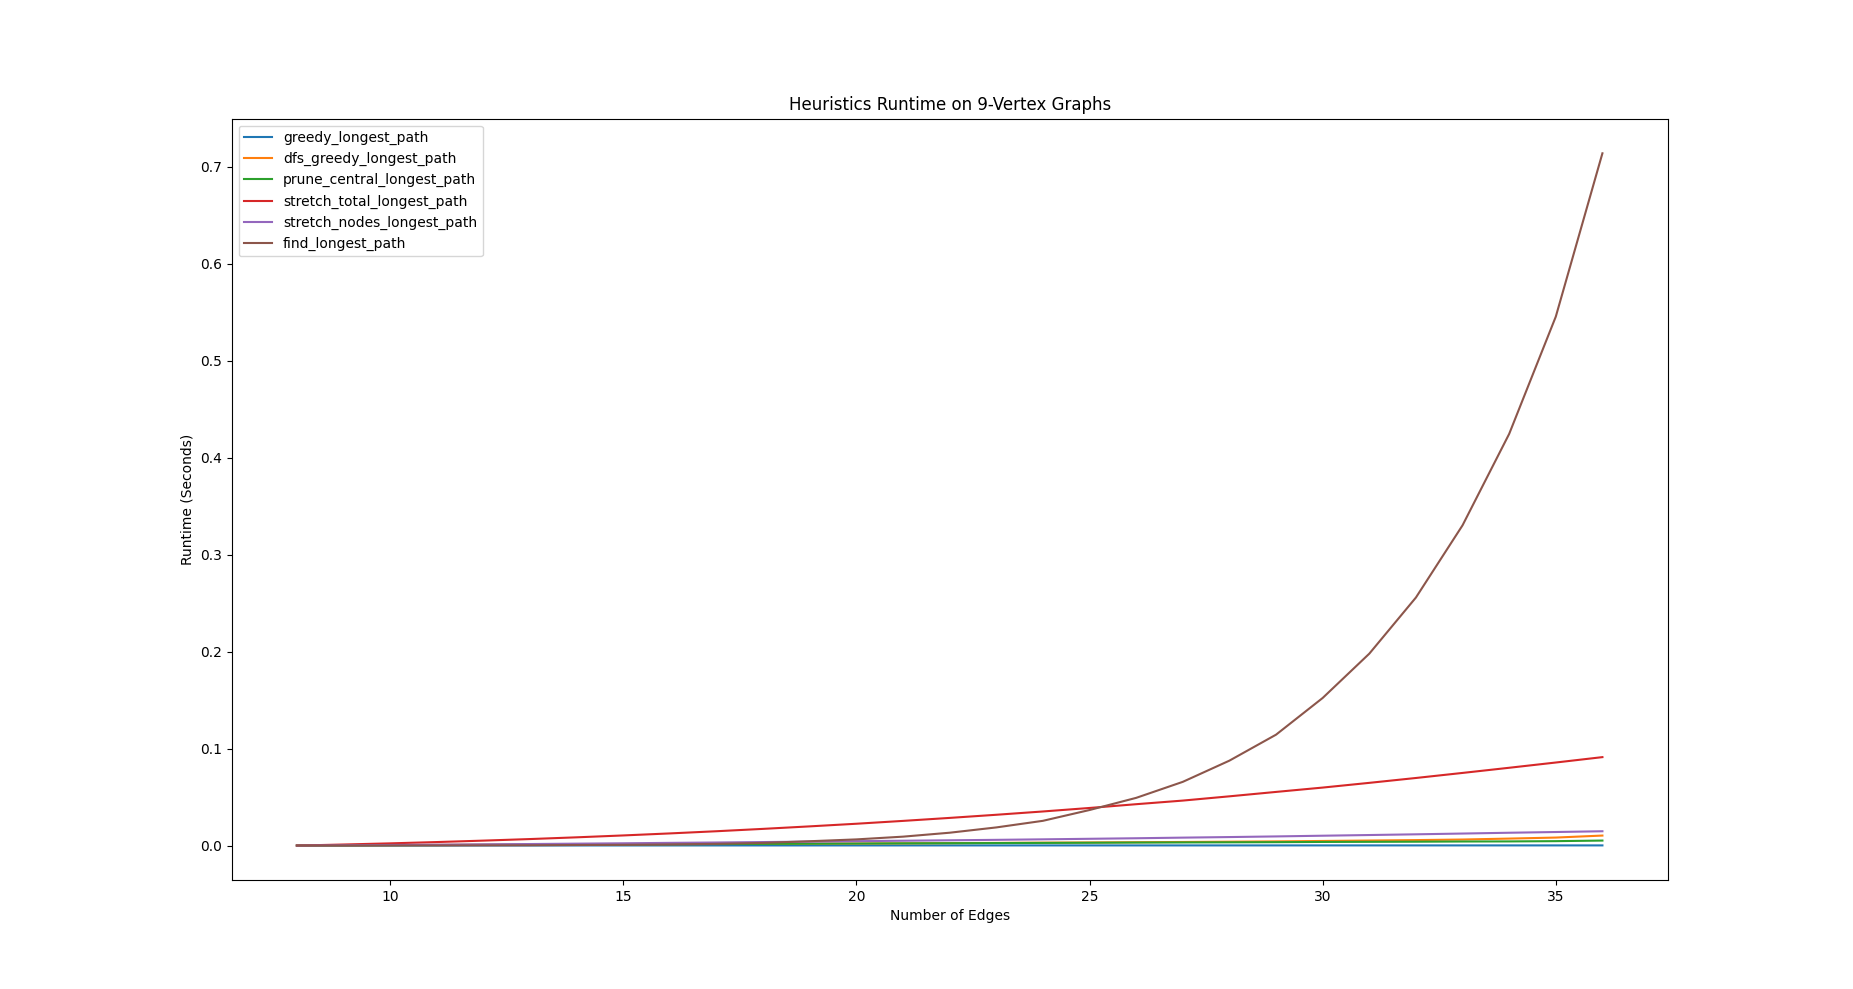
\includegraphics[width=\linewidth]{Runtime9VertexAll.png}
    \caption{Heuristics Runtime on Graphs with 9 Vertices}
    \label{fig:Runtime}
\end{figure*}

The accuracy benchmark confirmed the findings of several past experiments. All heuristics were seen to have a ``canyon'' behavior. At any vertex count, as the edge count increases, the accuracy of the heuristics decrease to a lower bound, then increases after hitting the lower bound. In other words, the LSP of tree graphs, and dense graphs were a accurately found by the heuristics, while the sparse and non-tree graphs were the difficult graphs to find a correct LSP for. This confirms the claims of other studies that have found the sparse graphs to be the real challenge instances for the LSP problem. 

In addition, the accuracy tests also revealed that both variants of the greedy algorithm, with and without the depth-first-search tiebreaker, were both guaranteed to get the correct LSP in dense graphs, which also confirms previous findings. For graph pruning, the accuracy shown was worse than the greedy heuristics, signalling that, as stand-alone heuristics, they are not as effective as greedy heuristics. However, it is possible that implementing them in tandem with something like A* or local search could produce desirable results.

The runtime tests we administered showed that in comparison to the naive, brute-force solution, all heuristic runtimes grew at a slower pace. The brute-force solution has a clear exponential growth in runtime as the number of edges increases, while the heuristics have runtimes that increase more gradually. The one exception to this behavior was the heuristic that stretched the graph periphery. Because of its need to loop through all edges each time, in sparse graphs, it has a slower runtime than the brute-force algorithm. Furthermore, as the number of vertices increased, the stretching heuristic's runtime also increased by a larger degree than other heuristics. Despite its relative inefficiencies, the stretching graph periphery heuristic was still more efficient than the naive solution.


\section{Conclusions}

The difficulties of the longest simple path problem are many and varied.
We explored possible implementations of heuristics for more efficient solutions or approximations to finding the LSP. Through our experimentation, we confirmed past findings about the greedy heuristics abilities to solve the LSP problem on dense graphs, and the difficulty that sparse graphs bring to the problem. We also discussed the reasoning behind the various graph pruning heuristics. While these heuristics have so far been less effective, there is still a large space to explore.

\section*{Acknowledgements}

I would like to thank Bart Massey and Cassaundra Smith for their help in the research into the longest path problem and writing of this paper. I would also like to thank Mark Galassi for providing the opportunity to be an intern at the Insitute for Computing in Research.

\bibliographystyle{plain}
\bibliography{References.bib}

\end{document}